\section{Schroeder}

Con l’obiettivo di ricreare passo dopo passo le unità descritte nell’articolo
\emph{Natural Sounding Artificial Reverberation}\footcite{ms:rev62}, le prime
implementazioni in \faust~sono relative ai due blocchi essenziali, \emph{Comb}
e \emph{All-Pass}.

\subsection{Comb}

Il codice di studio del filtro \emph{Comb} descritto in fig. \ref{fig:dfl}, con
i passi di correzione del dei tempi di integrazione per l'ottenimento della
risposta all'impulso indicata da Schroeder e riportata in fig. \ref{fig:dflir}.

\lstinputlisting{Code/dflc.dsp}

Il l'algoritmo utilizza le variabili $t$ (unità di tempo di ritardo espressa in
campioni) e $g$ (coefficiente di riscalamento del segnale in feedback).

\begin{figure}[htp]
\centering
\includegraphics[width=0.80\textwidth]{Code/dflc-svg/process.pdf}
\caption{delay feedback loop}
\label{fig:dflfaust}
\end{figure}

\subsection{All-Pass}

Il secondo algoritmo implementato permette di ottenere un filtro All-Pass
con risposta impulsiva in frequenza e ampiezza identiche a quelle descritte
dall'autore con figura \ref{fig:apf}

\lstinputlisting{Code/msapf.dsp}

Il comportamento All Pass è dato dalla somma del segnale ritardato scalato di
$(1-g^2)$ e il segnale diretto per $-g$, scalato con inversione di polarità.

\begin{figure}[htp]
\centering
\includegraphics[width=0.80\textwidth]{Code/msapf-svg/process.pdf}
\caption{\emph{All-Pass}}
\label{fig:apfaust}
\end{figure}

\subsection{Sequenza di All-Pass}

I filtri \emph{Comb} e \emph{All-Pass} implementati sono gli elementi basilari
della riverberazione artificiale di \ms. Di seguito espongo le implementazioni
articolate che l'autore espone dei filtri sopra descritti.

\lstinputlisting{Code/msapfseq.dsp}

\begin{figure}[htp]
\centering
\includegraphics[width=0.80\textwidth]{Code/msapfseq-svg/process.pdf}
\caption{Sequenza di \emph{All-Pass}}
\label{fig:apfseq}
\end{figure}

\subsection{Annidamento e controllo}

\ms, immediatamente dopo la creazione degli elementi base, una serie di risultati
sperimentali ottenuti nella ricerca della simulazione di alcuni dei comportamenti
del riverbero acustico. Uno di questi è la possibilità di annidare un \emph{All-Pass}
dentro un \emph{All-Pass} in modo che i due filtri combinati possano:
\begin{enumerate}
  \item bilanciare il rapporto tra segnale diretto e segnale riverberato
  \item l'introduzione di un ritardo tra i due segnali (diretto e riverberato)
  \item una dipendenza del tempo di riverberazione dalla frequenza
\end{enumerate}

\lstinputlisting{Code/msapfdwp.dsp}

\begin{figure}[htp]
\centering
\includegraphics[width=0.80\textwidth]{Code/msapfdwp-svg/process.pdf}
\caption{All-Pass contenente una unità comb contenente una unità all-pass}
\label{fig:apfdwp}
\end{figure}

\begin{figure}[htp]
\centering
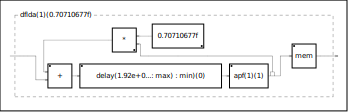
\includegraphics[width=0.80\textwidth]{Code/msapfdwp-svg/dflda-0x600001c847e0.pdf}
\caption{dfla: unità comb contenente un all-pass}
\label{fig:dfla}
\end{figure}

\subsection{Algoritmi Combinati}

Come già visto nel Capitolo 3, queste unità riverberanti non risultano particolaremente efficenti dal punto di vista della densità, se prese singolarmente, quindi il prossimo passo, come suggerito da Schroeder, è quello di crare delle reti di riverberatori combinando queste unità fondamentali.

\bigskip

Le due tipologie proposte consistono in una serie di All Pass connessi (figura \ref{fig:apfseq}), per la prima e, una serie di Comb connessi in cascata seguiti da 2 All Pass in serie, per la seconda.
Durante questa fase sono stati utilizzati numeri primi come valori dei ritardi in modo da evitare errori dovuti al campionamento.

L'algoritmo per la configurazione in serie risulta essere

\begin{code}
apfseq =  seq(i, 5, apf(ba.take(i+1, primet10),.7));
\end{code}

La lista ''primet10'' è stata caricata con i valori dei vari t. Come suggerito dall'autore, si è cercato di utilizzare numeri primi che mantenessero una relazione di $1/3$ l'uno dall'altro.
Il diagramma risultante è in figura \ref{fig:apfseqfaust}.

\begin{figure}[htp]
\centering
\includegraphics[width=%
0.90\textwidth]{apfseqfaust}
\caption{Sequenza di All Pass}
\label{fig:apfseqfaust}
\end{figure}

Il secondo algoritmo, per la configurazione `'Comb-All Pass'' vista in figura \ref{fig:comballpass}, è descritto nel seguente algoritmo

\begin{code}
reva((t,g,t1,g1),g2) = _<:_+(
    par(i,6, dflda(ba.take(i+1, t),G*ba.take(i+1,g))) :>
    seq(i, 2, apfn(ba.take(4-i, t1),G*ba.take(i+1,g1))))*(g2);
process = _ : reva((primetc1,combg1,primetc2,combg2),G);
\end{code}

`'par'' e `'rev'' sono rispettivamente, composizione parallela e composizione sequenziale e ci permettono di creare una cascata di 6 Comb seguita da una sequenza di 2 All Pass.

Il risultato è in figura \ref{fig:comballpassfaust}.

\begin{figure}[htp]
\centering
\includegraphics[width=%
1.2\textwidth]{comballpassfaust}
\caption{Algoritmo Comb-All Pass}
\label{fig:comballpassfaust}
\end{figure}

Quest'algoritmo risulta essere il più efficente ad ora e permette la riproduzione di oltre 1000 echi al secondo, un buon risultato considerando le stime effettute da Schroeder, ma che non corrisponde ad una riverberazione realistica e gradevole.
